\documentclass{article}
\usepackage{graphicx}
\usepackage{hyperref}
\usepackage{listings}

\title{Design and UI}
\author{Jake Hoogstrate}
\date{2/28/24}

\begin{document}
\maketitle

\section{Project Summary}
The goal of my project is to provide my client with an application that generates a course schedule based on a variety of user preferences. The data will be stored in a database so that it is saved, and the user will be able to edit it.

\section{Architecture}

\subsection{Chosen Architecture: Model-View-Controller (MVC)}
My project will follow the MVC architecture to separate concerns effectively.

\begin{itemize}
    \item \textbf{Model}: Manages faculty, courses, scheduling constraints, and global rules.
    \item \textbf{View}: Provides a graphical interface for interaction.
    \item \textbf{Controller}: Handles user inputs, logic, and interactions between Model and View.
\end{itemize}

\subsection{Main Modules}
\begin{itemize}
    \item \textbf{User Management Module} -- Handles faculty information storage and editing.
    \item \textbf{Course Management Module} -- Stores courses, allows additions, edits, and constraints.
    \item \textbf{Scheduling Engine} -- Implements logic to generate and optimize semester schedules.
    \item \textbf{GUI Module} -- Provides an interactive interface.
    \item \textbf{Data Import/Export Module} -- Supports bulk imports and generates formatted outputs.
    \item \textbf{Storage Module} -- Manages faculty, courses, and constraints in a database.
\end{itemize}

\subsection{Simplified Class Diagram}
\begin{itemize}
    \item \textbf{User} $\rightarrow$ interacts with \textbf{GUI}
    \item \textbf{GUI} $\leftrightarrow$ \textbf{Controller}
    \item \textbf{Controller} $\leftrightarrow$ \textbf{Model} (Faculty, Course, Schedule, Constraints)
    \item \textbf{Model} $\leftrightarrow$ \textbf{Database}
\end{itemize}

\section{Technology}

\textbf{Programming Language:}
\begin{itemize}
    \item Java (for backend logic and scheduling algorithm)
    \item JavaScript (for frontend interface)
\end{itemize}

\textbf{Frameworks:}
\begin{itemize}
    \item Frontend: React.js
    \item Database: Firebase
\end{itemize}

\section{Data Structure}

\subsection{Database Schema}
\begin{itemize}
    \item faculty: \{ id, name, time\_start\_preference, time\_end\_preference, num\_courses, preferred\_courses: [] \}
    \item courses: \{ id, name, credits \}
\end{itemize}

\section{Coding Standards}

\textbf{Database Naming Conventions:}
\begin{itemize}
    \item Table names in lowercase
    \item Column names in snake\_case
\end{itemize}

\textbf{Code Quality Standards:}
\begin{itemize}
    \item Follow typical Java naming conventions (PascalCase for classes, camelCase for methods and variables)
    \item Require unit tests for all modules, with \textbf{$>$50\%} test coverage before committing.
\end{itemize}

\section{User Interface Screens}

\begin{figure}[h]
    \centering
    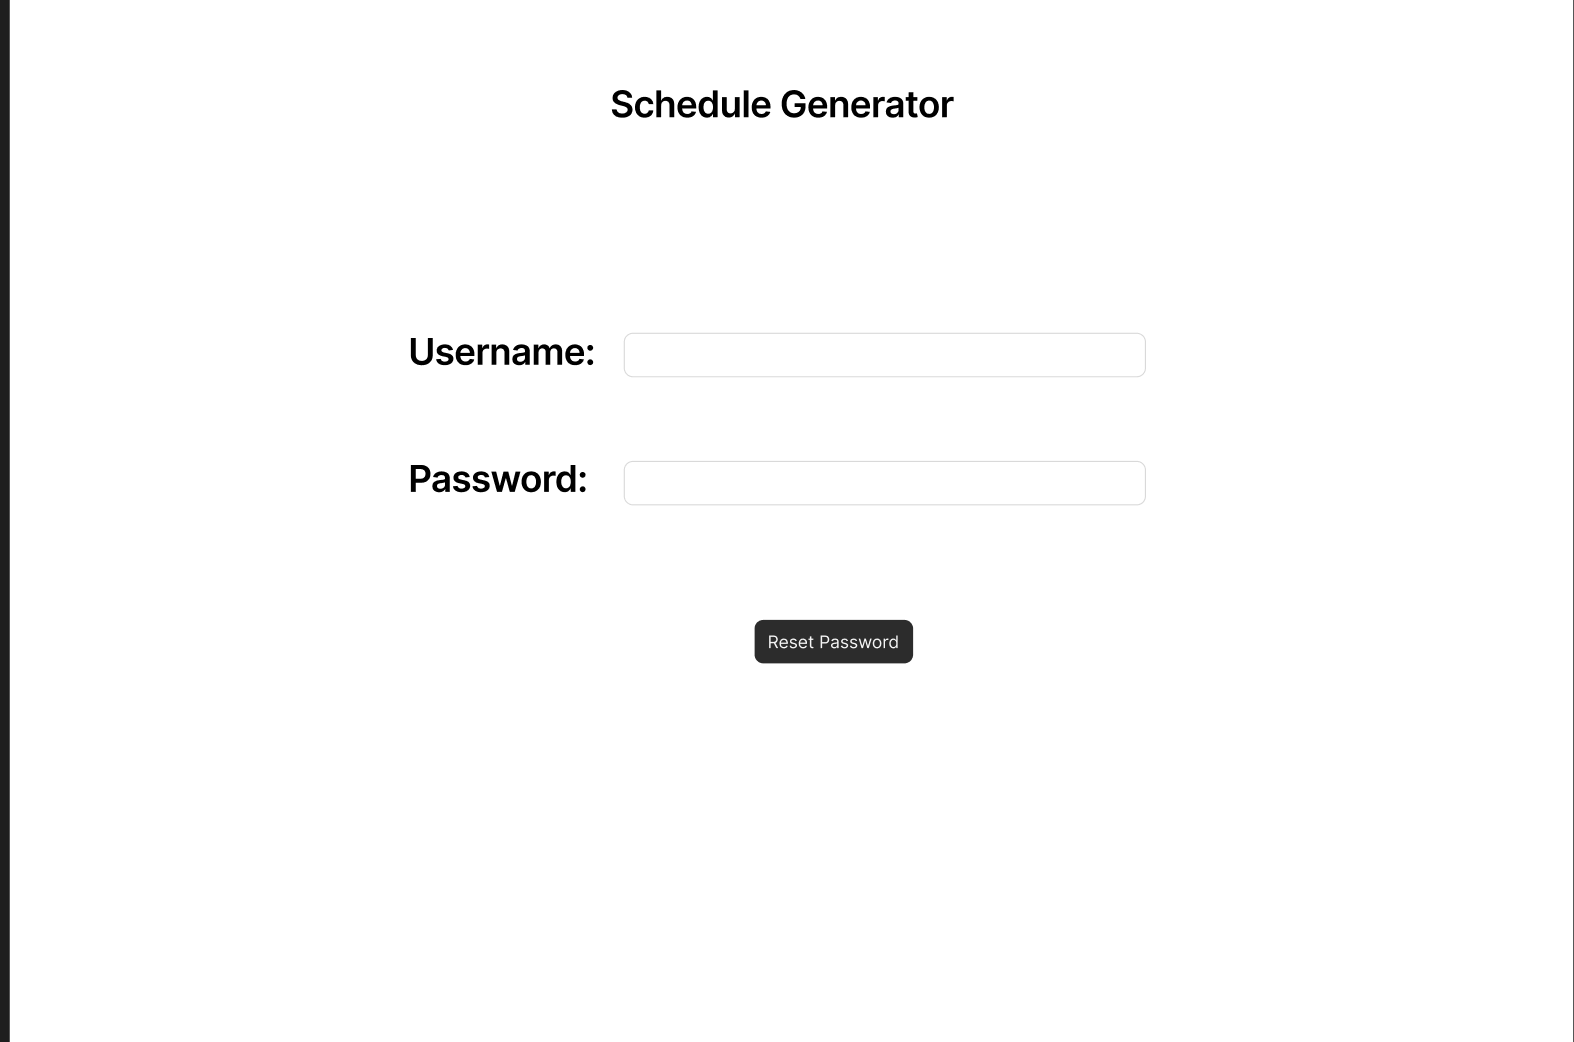
\includegraphics[width=0.8\textwidth]{photos/photo1.png}
    \caption{Login Screen}
\end{figure}

\begin{figure}[h]
    \centering
    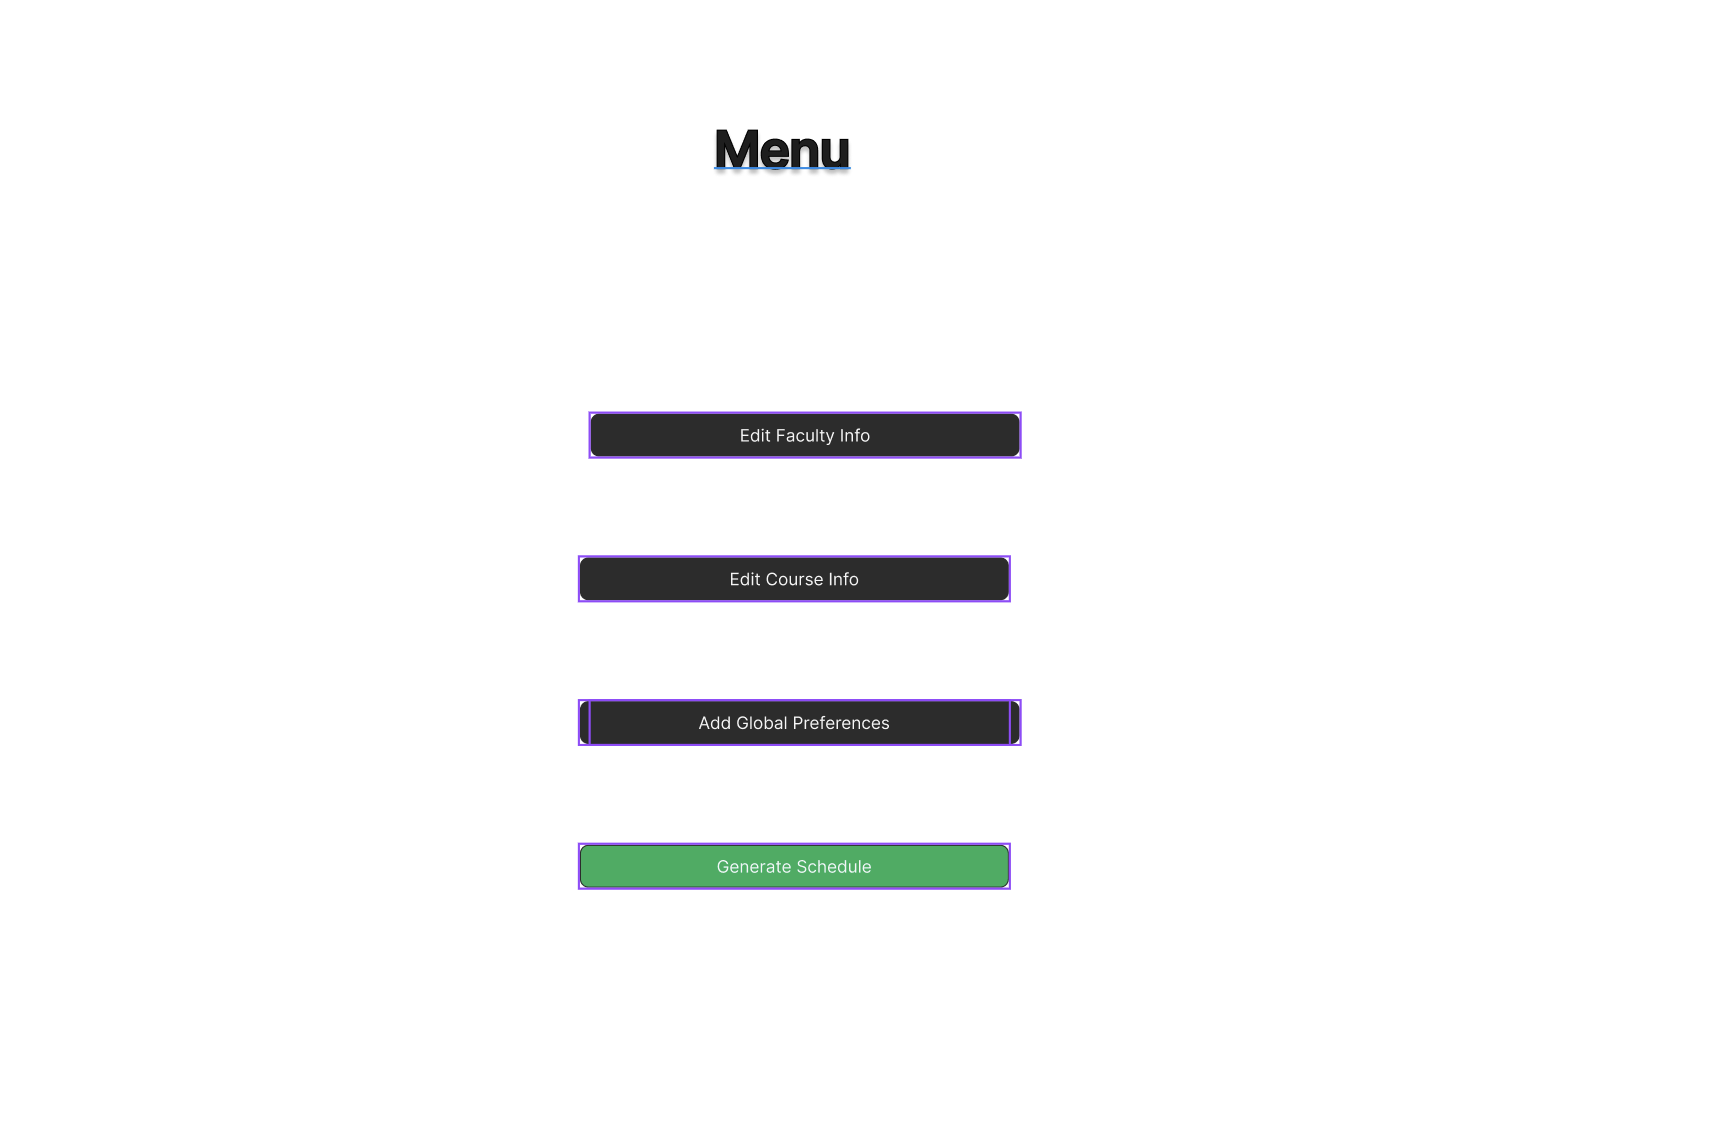
\includegraphics[width=0.8\textwidth]{photos/photo2.png}
    \caption{Main Menu}
\end{figure}

\begin{figure}[h]
    \centering
    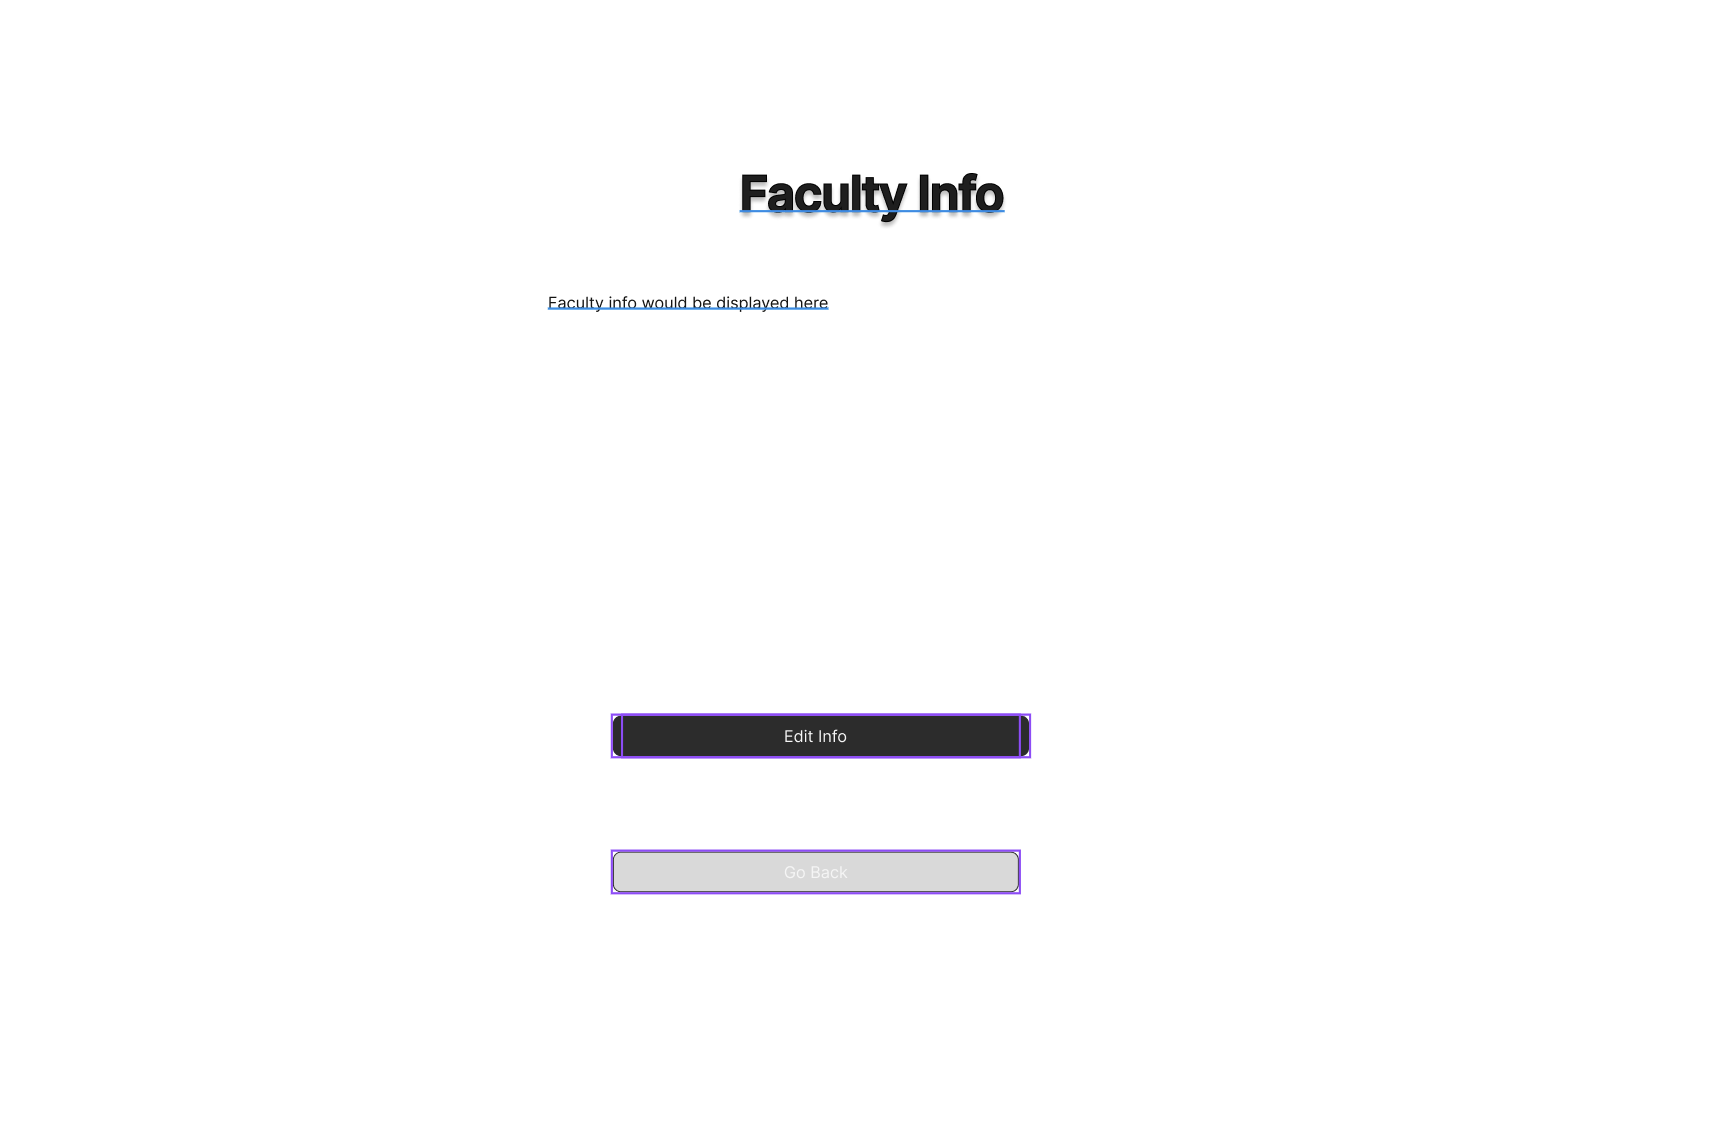
\includegraphics[width=0.8\textwidth]{photos/photo3.png}
    \caption{Faculty Information Screen}
\end{figure}

\begin{figure}[h]
    \centering
    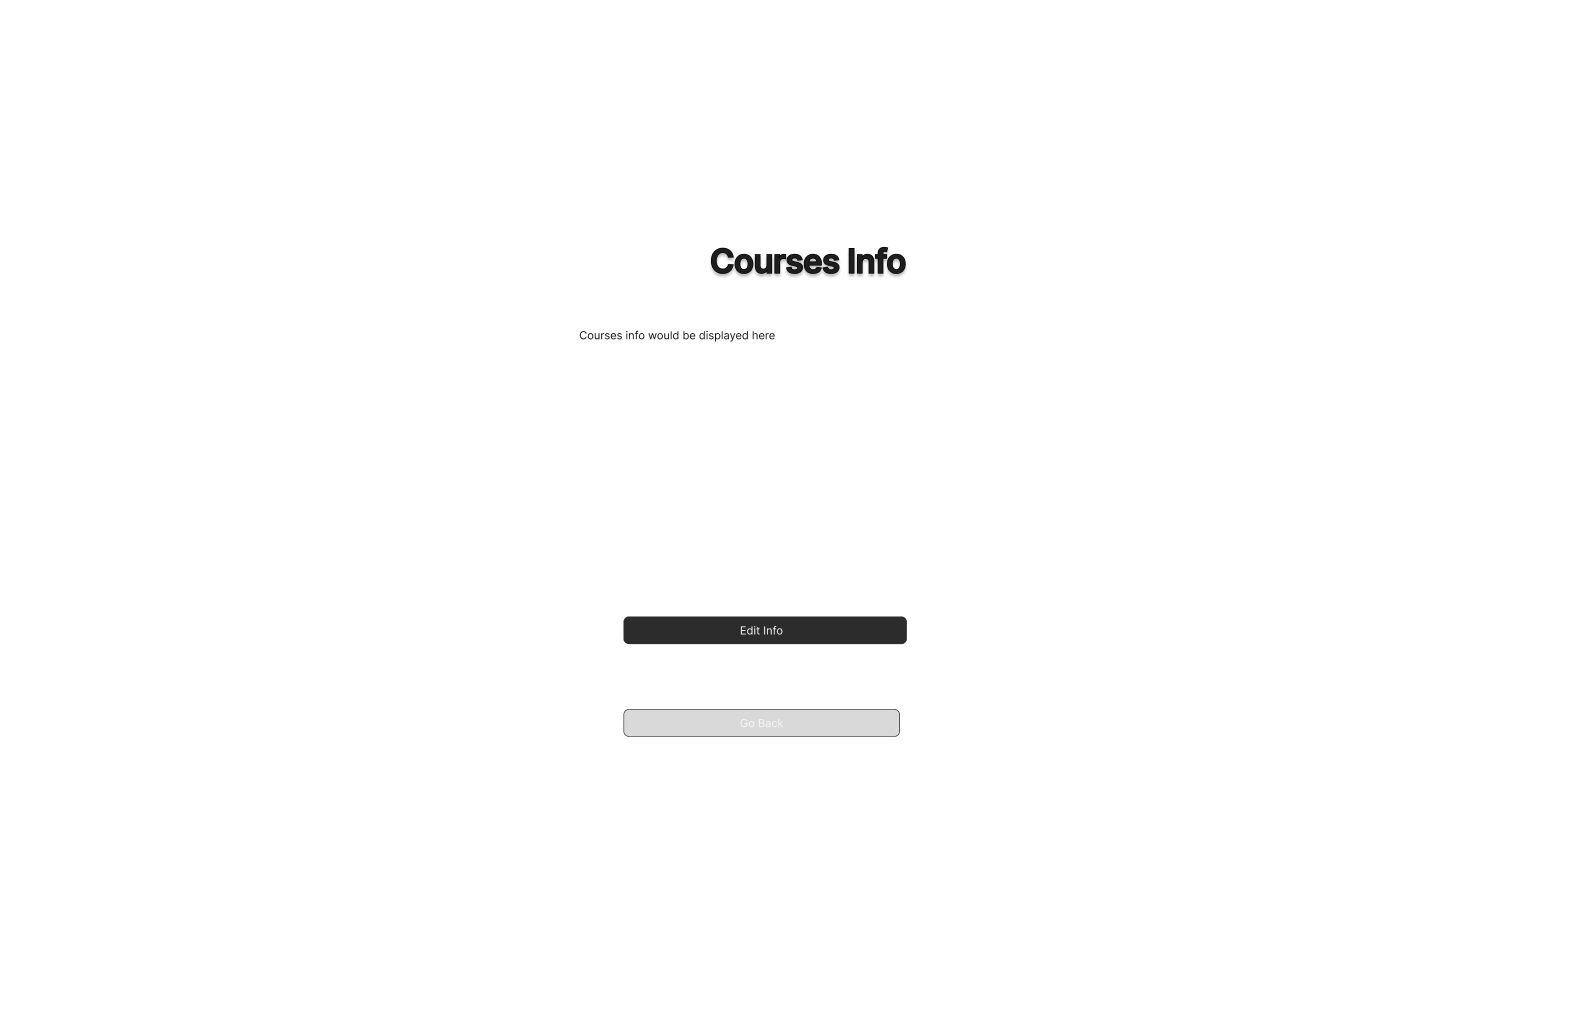
\includegraphics[width=0.8\textwidth]{photos/photo4.png}
    \caption{Course Information Screen}
\end{figure}

\begin{figure}[h]
    \centering
    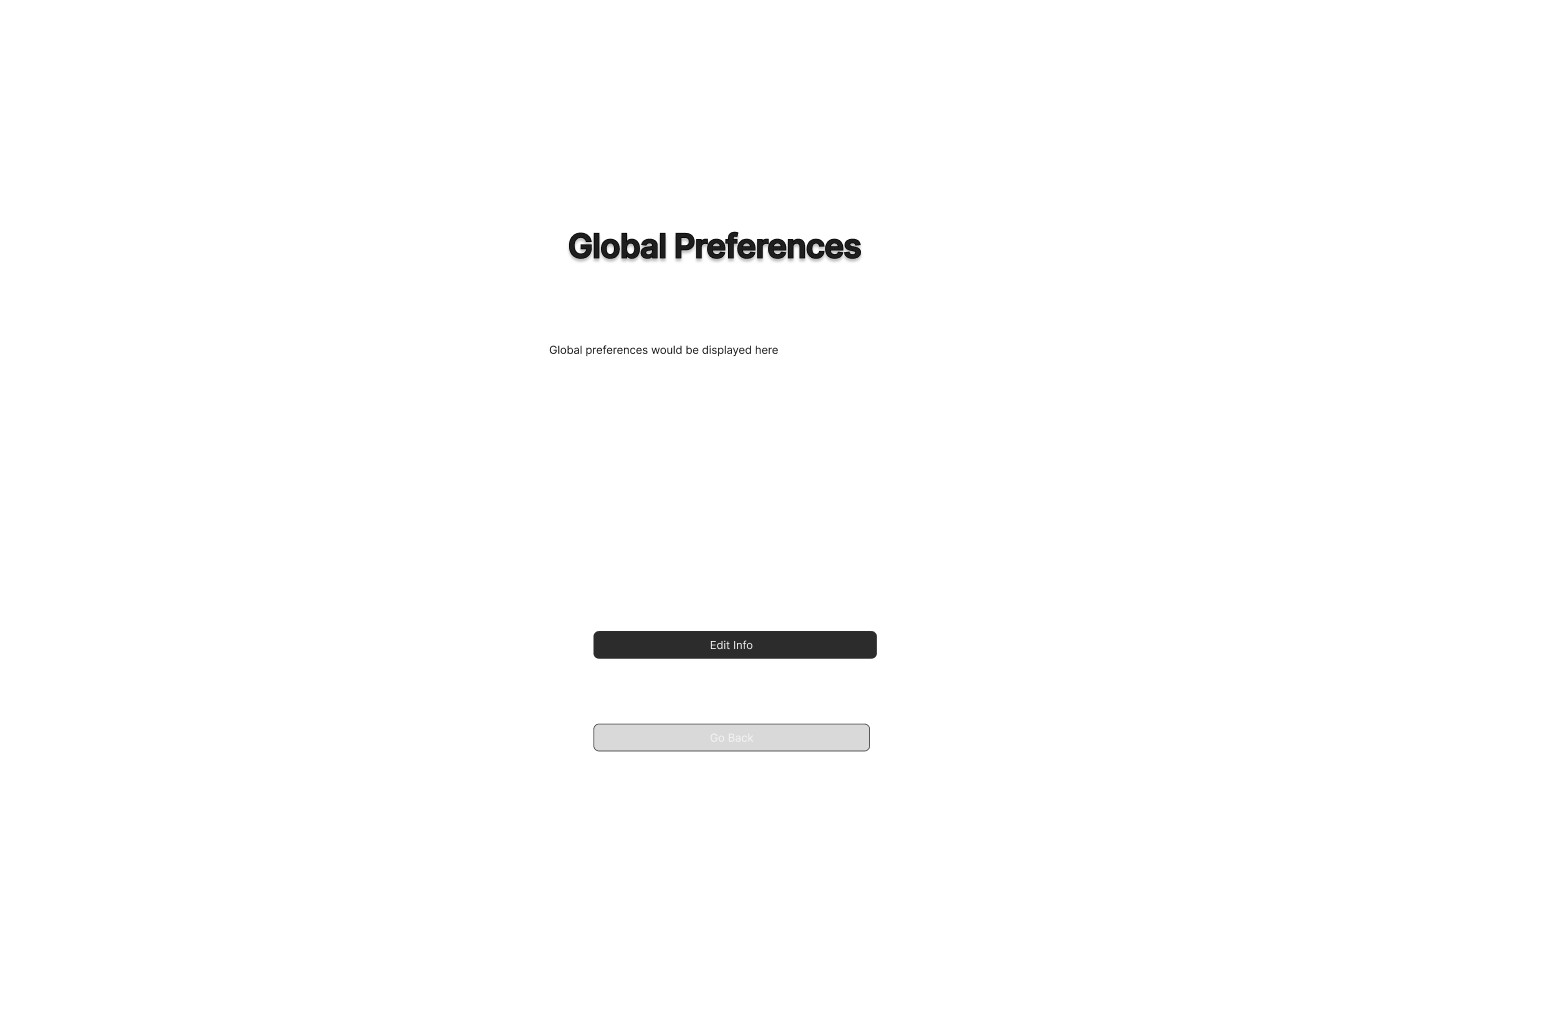
\includegraphics[width=0.8\textwidth]{photos/photo5.png}
    \caption{Schedule Screen}
\end{figure}

\begin{figure}[h]
    \centering
    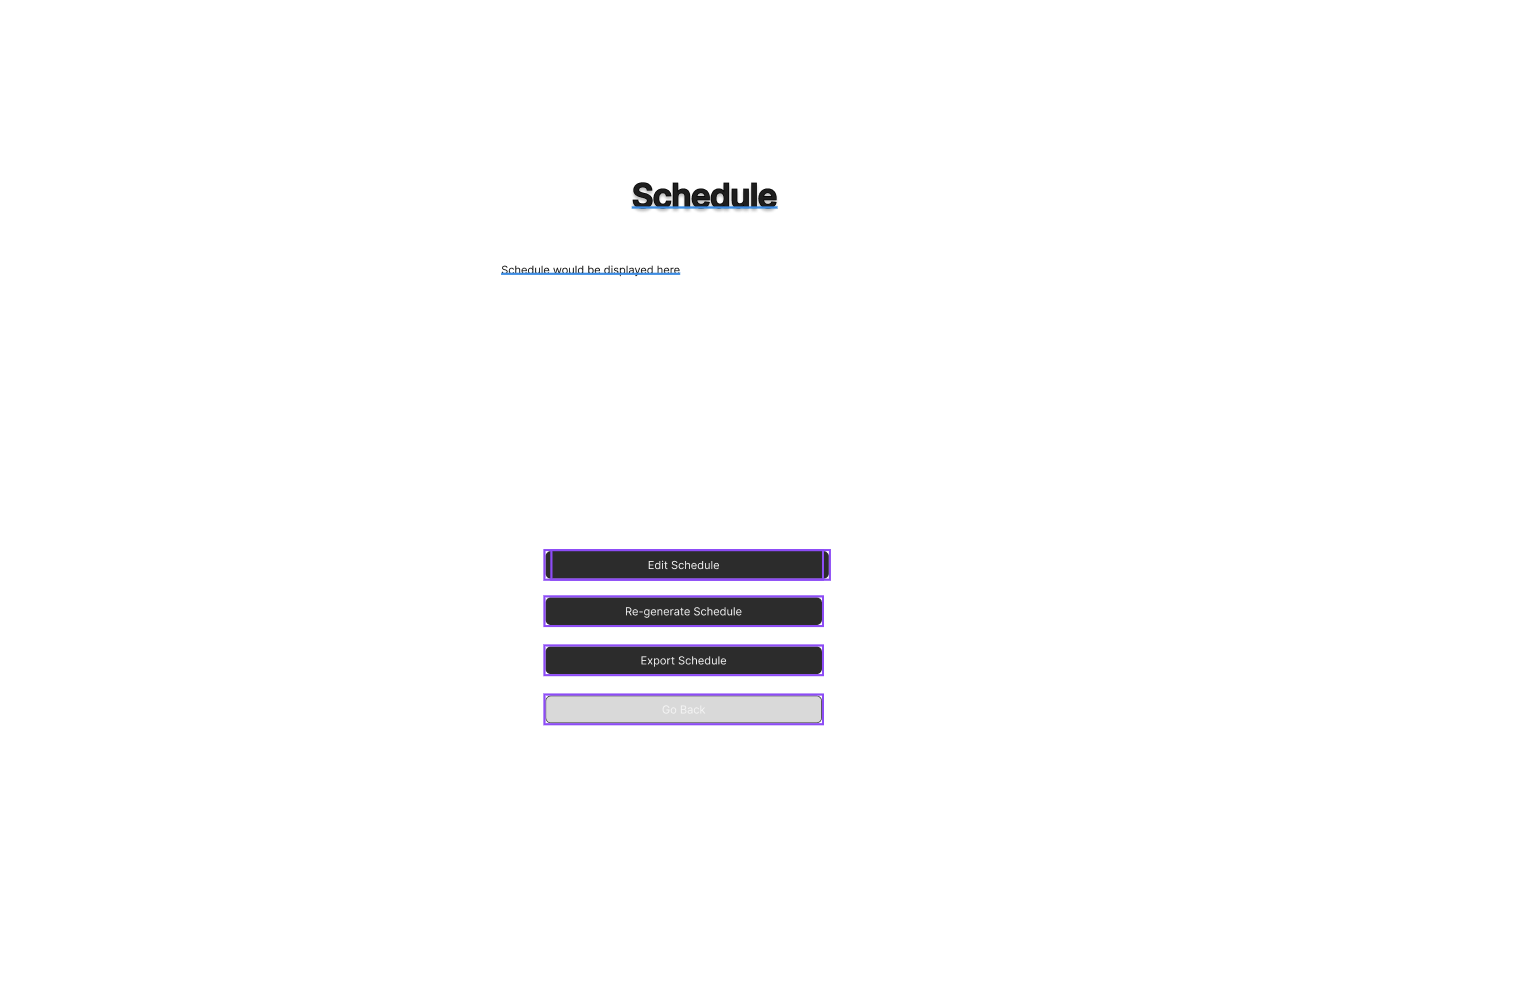
\includegraphics[width=0.8\textwidth]{photos/photo6.png}
    \caption{Export Schedule Screen}
\end{figure}

\begin{figure}[h]
    \centering
    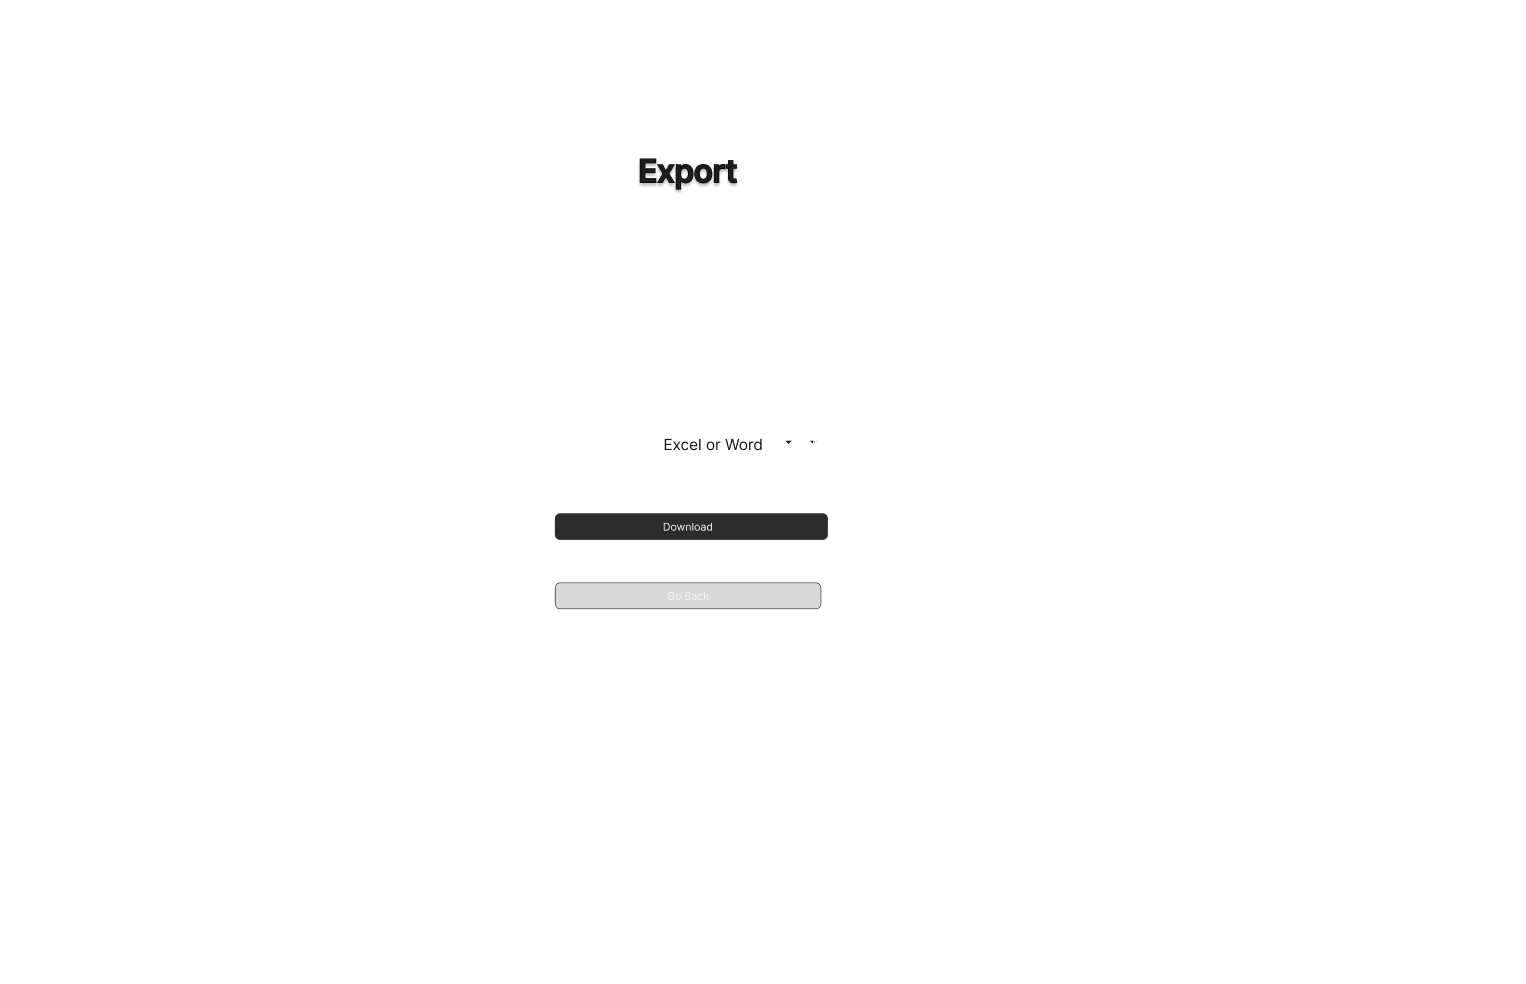
\includegraphics[width=0.8\textwidth]{photos/photo7.png}
    \caption{Global Preferences Screen}
\end{figure}

\end{document}

